% !TEX root = ./../../../_Thesis.tex

\begin{figure*}[!b]
	\centering

	\begin{tabular}{@{}r@{ } c@{ } c@{ } c@{ } c@{ } c }
	&
	\small{Synthetic} &
	\small{Synthetic } &
	\small{Camera} &
	\small{Camera Capture} &
	\small{Simulation} & 
	&
	\small{Input} &
	\small{Simulation} &
	\small{Capture} &
	\small{(+2.00 D)} &
	\small{} & \\

	\begin{sideways} \parbox[b]{20mm} {} \end{sideways} &
	
\includegraphics[width=0.185\textwidth]{__Images/05/WB_NCKZO_myopia/wb_N_20-200_Sloan@4x} &
	
\includegraphics[width=0.185\textwidth]{__Images/05/WB_NCKZO_myopia/wb_N_20-200_Sloan@4x+2,00D(simulated)} &
	
\includegraphics[width=0.185\textwidth]{__Images/05/WB_NCKZO_myopia/wb_N_20-200_Camera+0,00D} &
	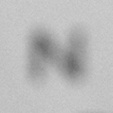
\includegraphics[width=0.185\textwidth]{__Images/05/WB_NCKZO_myopia/wb_N_20-200_Camera+2,00D(lens)} &
	
\includegraphics[width=0.185\textwidth]{__Images/05/WB_NCKZO_myopia/wb_N_20-200_Camera+2,00D(simulated)} \\

	\begin{sideways} \parbox[b]{20mm} {} \end{sideways} &
	
\includegraphics[width=0.185\textwidth]{__Images/05/WB_NCKZO_myopia/wb_C_20-200_Sloan@4x} &
	
\includegraphics[width=0.185\textwidth]{__Images/05/WB_NCKZO_myopia/wb_C_20-200_Sloan@4x+2,00D(simulated)} &
	
\includegraphics[width=0.185\textwidth]{__Images/05/WB_NCKZO_myopia/wb_C_20-200_Camera+0,00D} &
	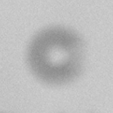
\includegraphics[width=0.185\textwidth]{__Images/05/WB_NCKZO_myopia/wb_C_20-200_Camera+2,00D(lens)} &
	
\includegraphics[width=0.185\textwidth]{__Images/05/WB_NCKZO_myopia/wb_C_20-200_Camera+2,00D(simulated)} \\
	
	\begin{sideways} \parbox[b]{20mm} {} \end{sideways} &
	
\includegraphics[width=0.185\textwidth]{__Images/05/WB_NCKZO_myopia/wb_K_20-200_Sloan@4x} &
	
\includegraphics[width=0.185\textwidth]{__Images/05/WB_NCKZO_myopia/wb_K_20-200_Sloan@4x+2,00D(simulated)} &
	
\includegraphics[width=0.185\textwidth]{__Images/05/WB_NCKZO_myopia/wb_K_20-200_Camera+0,00D} &
	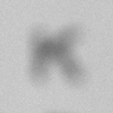
\includegraphics[width=0.185\textwidth]{__Images/05/WB_NCKZO_myopia/wb_K_20-200_Camera+2,00D(lens)} &
	
\includegraphics[width=0.185\textwidth]{__Images/05/WB_NCKZO_myopia/wb_K_20-200_Camera+2,00D(simulated)} \\
	
	\begin{sideways} \parbox[b]{20mm} {} \end{sideways} &
	
\includegraphics[width=0.185\textwidth]{__Images/05/WB_NCKZO_myopia/wb_Z_20-200_Sloan@4x} &
	
\includegraphics[width=0.185\textwidth]{__Images/05/WB_NCKZO_myopia/wb_Z_20-200_Sloan@4x+2,00D(simulated)} &
	
\includegraphics[width=0.185\textwidth]{__Images/05/WB_NCKZO_myopia/wb_Z_20-200_Camera+0,00D} &
	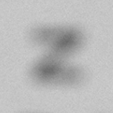
\includegraphics[width=0.185\textwidth]{__Images/05/WB_NCKZO_myopia/wb_Z_20-200_Camera+2,00D(lens)} &
	
\includegraphics[width=0.185\textwidth]{__Images/05/WB_NCKZO_myopia/wb_Z_20-200_Camera+2,00D(simulated)} \\
	
	\begin{sideways} \parbox[b]{20mm} {} \end{sideways} &
	
\includegraphics[width=0.185\textwidth]{__Images/05/WB_NCKZO_myopia/wb_O_20-200_Sloan@4x} &
	
\includegraphics[width=0.185\textwidth]{__Images/05/WB_NCKZO_myopia/wb_O_20-200_Sloan@4x+2,00D(simulated)} &
	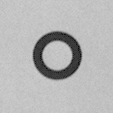
\includegraphics[width=0.185\textwidth]{__Images/05/WB_NCKZO_myopia/wb_O_20-200_Camera+0,00D} &
	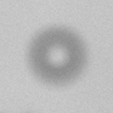
\includegraphics[width=0.185\textwidth]{__Images/05/WB_NCKZO_myopia/wb_O_20-200_Camera+2,00D(lens)} &
	
\includegraphics[width=0.185\textwidth]{__Images/05/WB_NCKZO_myopia/wb_O_20-200_Camera+2,00D(simulated)} \\

	\end{tabular}
	
	\caption[Comparisons of our simulated results against ground truth obtained with a myopic camera]{Comparisons of our simulated results against ground truth obtained with a myopic camera. 
		The first two columns show synthetic images and the results of their simulations for +2.0408 D of myopia. The last three columns show, respectively, images captured by the DSLR camera, images captured by the DSLR camera with an additional +2.0 D lens, and the results of our simulations for +2.0408 D of myopia applied to the images shown in the column {\it Camera Capture}.}
	\label{fig:myopia_nckzo_wb}
\end{figure*}
